
In our experiments, we evaluated our indexing techniques on two real world datasets. We have compared our indexing techniques by comparing the running time with that of the state of the art technique . We are also concerned about the indexing time, especially for the M-tree index structure since we do not want our index procedure to run into hours.

The first dataset is the Swamidass dataset . The second dataset is from DUD, a directory of useful decoys for benchmarking virtual screening. DUD is provided by the Shoichet Laboratory in the Department of Pharmaceutical Chemistry at the University of California, San Francisco (UCSF). DUD is derived from ZINC, a database of commercially avaiilable compounds. To extarct fingerprints we used MOLPRINT2D, a molecular fingerprinting technique.


\section{M-tree Indexing analysis}	

For these set of experiments the test bed used was a 4 Intel(R) Core(TM) i7-4770 CPU \@ 3.40GHz with 8GB RAM. We have varied several parameters in the experiment and have tried to estimate them emperically. We have used the Swamidass dataset for all analysis of the M-tree. We use different dataset sizes of 1000, 10,000 and 100,000 number of chemical compounds.

For evaluation purposes we implemented a linear brute force scan to compute the range query and used that as a benchmark for the results. The result set obtained from our technique was compared with the linear brute scan answer set for verification purposes using the fingerprint id's. The query time and the indexing time is averaged over the 500 random query sample data points and the unit in ms per compound. We have varied the following parameters .


\subsection{Limiting Outlier Set Size }

It is the Minimum limiting size of the outlier set allowed (o). When the outlier set size falls below this limit, we terminate the indexing process.

\begin{figure}[ht]	
\centering
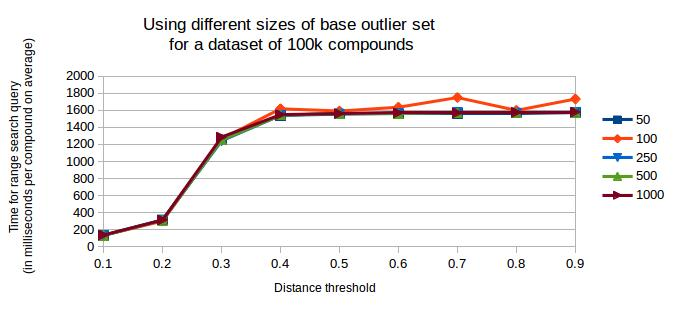
\includegraphics[width=1 \columnwidth]{img/image1.jpg}
\caption{Average Range Search Query time versus Distance Threshold for various sizes of base outlier set}
\label{fig:5.1}
\end{figure}

As seen in \ref{fig:5.1} we can observe that the range search query time is almost constant with change in number of limiting outlier set size. We observed that the outlier base size did not have a significant effect on the query time for range search or on the number of comparisons. The indexing time increases with a lesser outlier base size because the depth of the M-tree increases . The algorithm is applied recursively on the outlier sets, hence when we have a lower base size limit for the outlier sets the number of times the recursion is applied is greater. Since we did not see a great change in query time or number of comparisons we have fixed the size the outlier size limit to 1/100th of the dataset size for all the future experiments described below.
\begin{figure}[ht]	
\centering
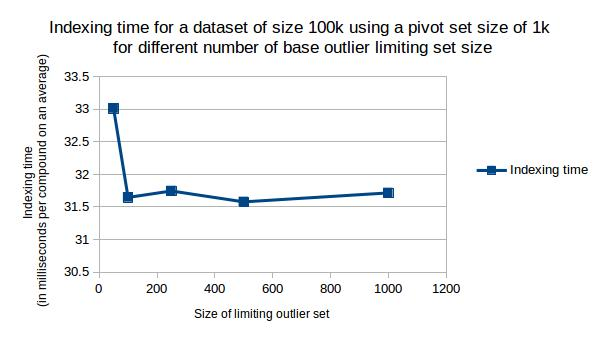
\includegraphics[width=1 \columnwidth]{img/image8.jpg}
\caption{Indexing time versus different sizes of base limiting outlier set}
\label{fig:5.2}
\end{figure}
\begin{enumerate}

	\item No. of random pivots chosen at each step of the indexing process (p). \textit{p} determines the number of nodes at every level of the index structure. The number of nodes at each level is equal to p+1.

	\item The range query distance threshold (t)	is thse cutoff used for determining similarity.\\
\end{enumerate}




\subsection{Pivot Set size}

\subsection{Threshold Distance}

\begin{figure}[ht]	
\centering
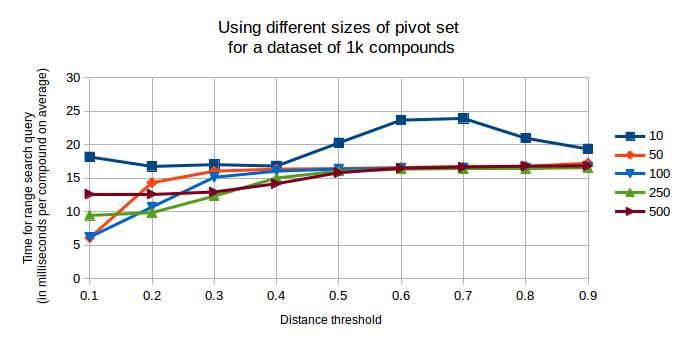
\includegraphics[width=1 \columnwidth]{img/image2.jpg}
\caption{Average Range Search Query time versus Distance Threshold for various sizes of pivot set - 1k database}
\label{fig:5.2a}
\end{figure}


\begin{figure}[ht]	
\centering
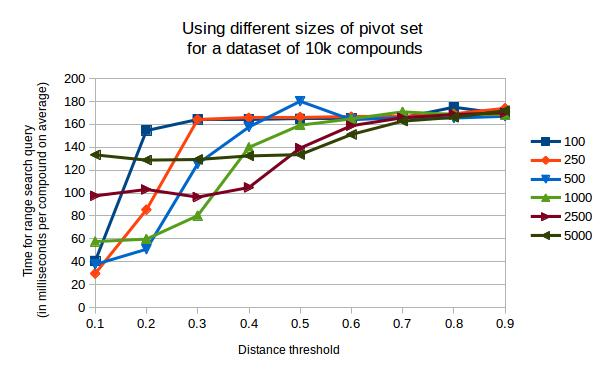
\includegraphics[width=1 \columnwidth]{img/image3.jpg}
\caption{Average Range Search Query time versus Distance Threshold for various sizes of pivot set - 10k database}
\label{fig:5.3}
\end{figure}


\begin{figure}[ht]	
\centering
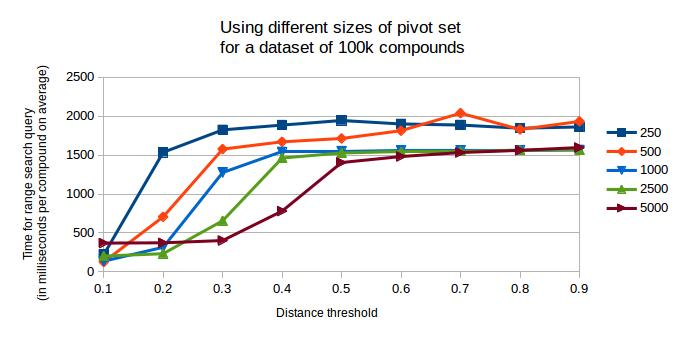
\includegraphics[width=1 \columnwidth]{img/image4.jpg}
\caption{Average Range Search Query time versus Distance Threshold for various sizes of pivot set - 100k database}
\label{fig:5.4}
\end{figure}



\begin{figure}[ht]	
\centering
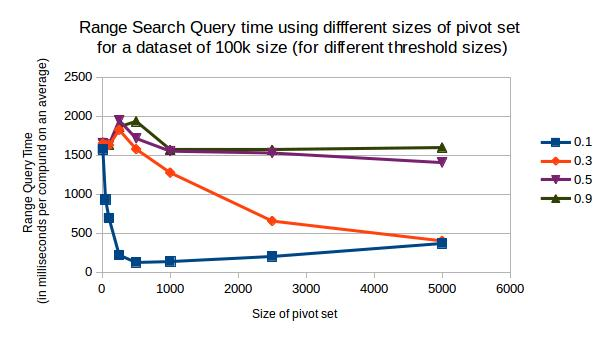
\includegraphics[width=1 \columnwidth]{img/image5.jpg}
\caption{Average Range Search Query time versus various sizes of pivot set for different theshold distances}
\label{fig:5.5}
\end{figure}



\begin{figure}[ht]	
\centering
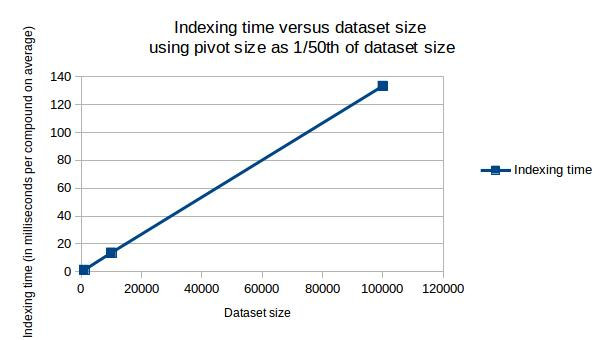
\includegraphics[width=1 \columnwidth]{img/image6.jpg}
\caption{Indexing time versus dataset size}
\label{fig:5.6}
\end{figure}



\begin{figure}[ht]	
\centering
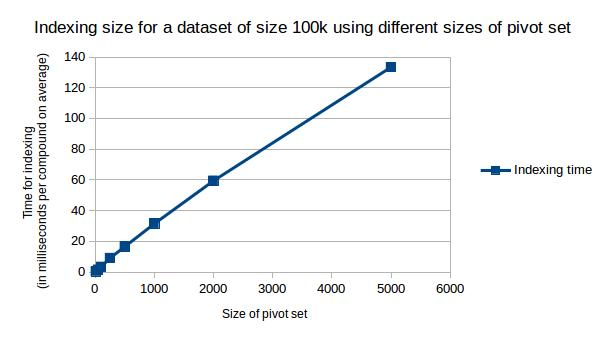
\includegraphics[width=1 \columnwidth]{img/image7.jpg}
\caption{Indexing time versus different sizes of pivot set size}
\label{fig:5.7}
\end{figure}



